\chapter{Conclusioni}
\label{Cha:conclusioni}
\thispagestyle{empty}

L'ultimo capitolo fornisce una sintesi dei risultati ottenuti e alcuni suggerimenti su possibili problematiche che potrebbero essere risolte in futuro.

\section{Risultati ottenuti}
I risultati sperimentali hanno rilevato che il sistema è in grado di acquisire correttamente le \textit{point cloud} dei battistrada e che gli algoritmi possono effettuare misurazioni, identificare le scanalature e misurarne la profondità.\\
\newline
Riprendendo i test effettuati nel paragrafo \ref{performance}, riportiamo i risultati delle scansioni riguardante il battistrada di tipo \textit{2}:

\begin{table}[H]
\centering
\begin{tabular}{||c c c c||} 
 \hline
 N & min (mm) & max (mm) & avg (mm) \\ [0.5ex]
 \hline\hline
 1 & 0.50 & 4.85 & 2.68 \\ 
 \hline
 2 & 0.50 & 4.73 & 2.62 \\
 \hline
 3 & 0.51 & 4.76 & 2.64 \\
 \hline
 4 & 0.51 & 4.80 & 2.66 \\
 \hline
 5 & 0.50 & 4.85 & 2.68 \\
 \hline
 6 & 0.50 & 4.77 & 2.64 \\
 \hline
 7 & 0.51 & 4.82 & 2.67 \\
 \hline
 8 & 0.50 & 4.82 & 2.66 \\
 \hline
 9 & 0.50 & 4.79 & 2.65 \\
 \hline
 10 & 0.51 & 4.80 & 2.66 \\
 \hline
\end{tabular}
\caption{Valori calcolati su una serie di misurazioni del battistrada di tipo 2.}
\label{table:1}
\end{table}

\noindent Ogni misura calcolata dal programma è stata verificata direttamente sugli pneumatici utilizzando un calibro. Nonostante il punto di profondità massima cambiasse leggermente posizione, le misurazioni sono risultate abbastanza accurate e i test hanno sancito il raggiungimento dell'obiettivo che ci si era posti per il progetto.\\

\begin{figure}[H]
	\centering
	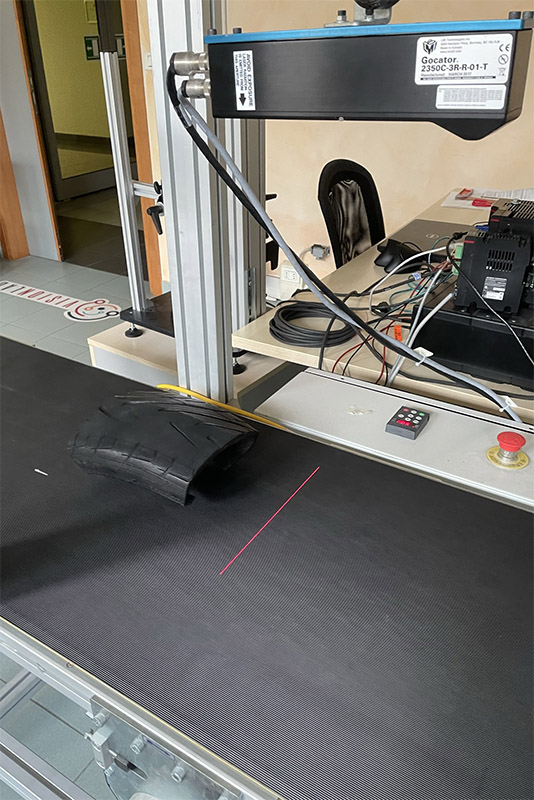
\includegraphics[width=0.40\columnwidth]{./pictures/gocator_conveyor_1.jpg}
	\hspace{1em}
	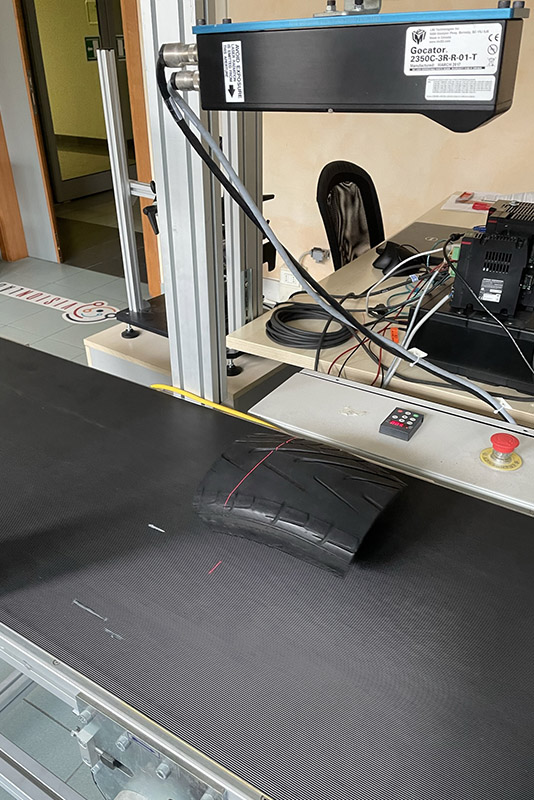
\includegraphics[width=0.40\columnwidth]{./pictures/gocator_conveyor_2.jpg}
	\caption{Il Gocator in azione durante una scansione.}\label{fig:gocator_conveyor}
\end{figure}

\section{Conclusione e lavori futuri}
Grazie allo studio di questa materia e al rispettivo progetto d'esame, è stata esplorata una branca dell'intelligenza artificiale molto importante per la moltitudine di benefici che apporta in tutti i settori per migliorare l'esperienza del consumatore, ridurre i costi e aumentare la sicurezza.\\
\newline
Seppure i risultati ottenuti sono risultati molto buoni, il margine di miglioramento è ampio, ed una futura ottimizzazione degli algoritmi e di altri particolari del Gocator, potrebbe portare a risultati ancora migliori.

\nocite{opencv_library}
\nocite{helix_toolkit_documentation}
\nocite{wpf_whatis}
\nocite{wrapping_whatis}
\nocite{dll_whatis}
\nocite{direct_industry}
\nocite{redazione_geomedia}
\nocite{lmi_technologies}
\nocite{image_s_blog}
\nocite{point_cloud_library_1}
\nocite{point_cloud_library_2}
\nocite{point_cloud_library_3}
\nocite{point_cloud_library_4}
\nocite{the_gsl_team}
\nocite{wang2019}
\nocite{booksdaglib0034531}
\nocite{gonzalez2008digital}
\nocite{named_pipe_whatis}